%\documentclass[12pt,a4wide]{article}
\documentclass[12pt]{report}
\setlength{\parindent}{0in}
\setlength{\parskip}{2mm}
\usepackage{latexsym,a4wide}
\usepackage{ifpdf}
\usepackage{tabularx}
\usepackage{multicol}
\usepackage{fancyhdr}
\usepackage[table,xcdraw]{xcolor}
\ifpdf
    \usepackage[pdftex]{graphicx}   % to include graphics
    \pdfcompresslevel=9
    \usepackage[pdftex,     % sets up hyperref to use pdftex driver
            plainpages=false,   % allows page i and 1 to exist in the same document
            breaklinks=true,    %i link texts can be broken at the end of line
            colorlinks=true,
            colorlinks=false,
            pdftitle=Katabasis
            pdfauthor=Gruppe 6.1
           ]{hyperref}
    \usepackage{thumbpdf}
\else
    \usepackage{graphicx}       % to include graphics
    \usepackage{hyperref}       % to simplify the use of \href
\fi

%02122 Fagprojekt
\title{02122 Project course, Spring 2014 \\
DTU Compute \\
Technical University of Denmark \\~\\~\\ Katabasis \\ Group 6.1}
\author{s113414 Cebrail Erdogan \\
        s123062 Carsten Nielsen \\
        s123094 Jonathan Becktor\\
        s123995 Philip Berman   \\  }
        \date{\today}
\begin{document}


\pagestyle{headings}



\maketitle

\begin{abstract}
Using the Arduino hardware with Gameduino 2, we will create an advanced game.
The game will have elements as AI and Map generation.
Coding in arduinos environment and make it work in the
limited hardware is quite a challenge and fun.
\end{abstract}


\tableofcontents

\newpage

%\section{Introduction}
\chapter{Introduction}
The main purpose of the project is to make an advanced game using the Arduino hardware.
Arduino is a programmable piece of hardware. Combining it with the  Gameduino 2 makes
it possible for us to create a rich game. The Gameduino extends the Arduino with a
touch screen, extra space and processing power.
\section{Arduino}
Programming an Arduino is done in its own language, simply named \emph{Arduino programming language}\footnote{http://www.arduino.cc/}. It is based off Wiring, and is reminiscent of both C and C++, but is neither. The IDE is based off the Processing IDE. This mix of languages and sparse documentation makes it difficult for the programmer, even though the Arduino was meant to ease newbies into programming. An example, would be the keyword {\tt new}, which officially is not supported\footnote{The official reference page http://arduino.cc/en/Reference/HomePage does not include the keyword.}. This is confusing, because {\tt new} is completely functional, even syntax highlit. It instantiates an object in the heap rather than the stack, and returns the pointer to this object. Other unlisted keywords we found during development were delete, remove, size, update, speed, move and clear.\\ %Carsten
Our arduinos and their technicalities
\section{Gameduino 2}
The gameduino and technicalities.

\newpage

\chapter{Problem Analysis and Requirements specification}

Even before we got the Arduino leonardo, we knew that it could cause trouble. None of had experience in this unit and
we had never tried to code in a unit with a 'simple'
microprocesser like this one.

We were sure that the limited power and space capacitywould be a challange. Another thing was its IDE. The Arduino IDE has its own language (based on c/c++), which was not the most
sophisticated language according to what we heard. We did neither have any kind of emulator, which we definitely would have used, before getting the unit in our hands.

We were also sceptical about what Gameduino 2 was capable of. The examples
which were shared through their site\footnote{http://excamera.com/sphinx/gameduino2/} did not look impressing. Only one of them
looked like an advanced game.

As we did not have any experience with these units, we were also unsure of how to connect them. Do we need to do any soldering? or but any extra equipment?

\newpage

\section{Gameplay}%Jonathan Philiph
We originally wanted to implement a rpg style platformer with: "items, hero leveling, abilities and a story."

We decided to create a "rogue like" game and focus on increasing difficulty per level and having a high score as the intensive to play the game.

We want simple yet easily recognizable imagery. Animations should include smooth transitions and it should be easy for the player to feel like he or she is truly in control of their character's actions in the game. There shouldn't be any points in gameplay where it's confusing as to what exactly is happening on screen. Essentially the game should look nice but still keep the sense of retro genre game.

High scores is something you almost always see in arcade games or just smaller games. Its a great way to compare and compete and to show who's the best.

Coin were added as an additional game play element to broaden the game. The player now has an incentive to go explore the entirety of the map, since collecting coins is an easy way to get additional score.


\include{Preliminaries_theory}

%Be more precise about what the system should and should not satisfy.
%Be sure to use the vocabulary introduced in the problem analysis.
\chapter{Requirements specification}

\subsection{Gameplay}%Jonathan
We originally wanted to implement a rpg style platformer with:
\begin{enumerate}
\item Items
\item Hero leveling
\item Abilities
\item A decent story
\end{enumerate}
We quickly found out that the limited flash memory on the arduino would greatly limit what we could implement. We agreed on going back to the classics of arcade games. We decided to create a "rogue like" game and focus on increasing difficulty per level and having a high score as the intensive to play the game.

\subsubsection{High Score}
High scores is something you almost always see in arcade games or just smaller games. Its a great way to compare and compete and to show who's the best.
To do this we were requierd to save data on the EEPROM which is the ´hard drive` of the arduino. This way the high score will never reset unless we want it to.

\subsubsection{Coins}
Coin were added as an additional game play element to broaden the game. The player now has an incentive to go explore the entirety of the map, since collecting coins is an easy way to get additional score.

%Discuss how development processed, problems encountered and how some features were cut or added.
\chapter{Development Process} %Carsten
Development started the 17th of February and ended the 19th of June, with three week period ranging from 4th to 19th of June. Up until the three period we met once a week, and thereafter met daily. We attempted to distribute work equally, but each of us programmed and wrote about specific parts of the project.

\section{Timeplan} %Cebrail/Jonathan
When we started the project we created a waterfall chart containing our plans for every week. The waterfall chart is a sequential design process. It is designed to get through the project phases and have a product as soon as possible. The phases in our project can be seen in the figure below.
\newline
As we revisited our waterfall model throughout development, our main time plan can be considered to be iterative. The revisits have mainly been to extend features,debugging or optimizing.
\newline
When the waterfall ends and we still have time we will go back and visit the steps and check for new requirements.
\newline
The waterfall gives a good picture of the big phases, but the pre-planned week schedules are not always much help, as they are not dynamic. We can't reconstruct our waterfall every time we meet a conflict. This is here where the timeboxes are handy, which is used to the most detailed part of the time planning - see next subsection. You can check our waterfall timeplan in the appendices, please see Figure~\ref{fig:Waterfall_chart} for that.
\begin{figure}[h]
\centering
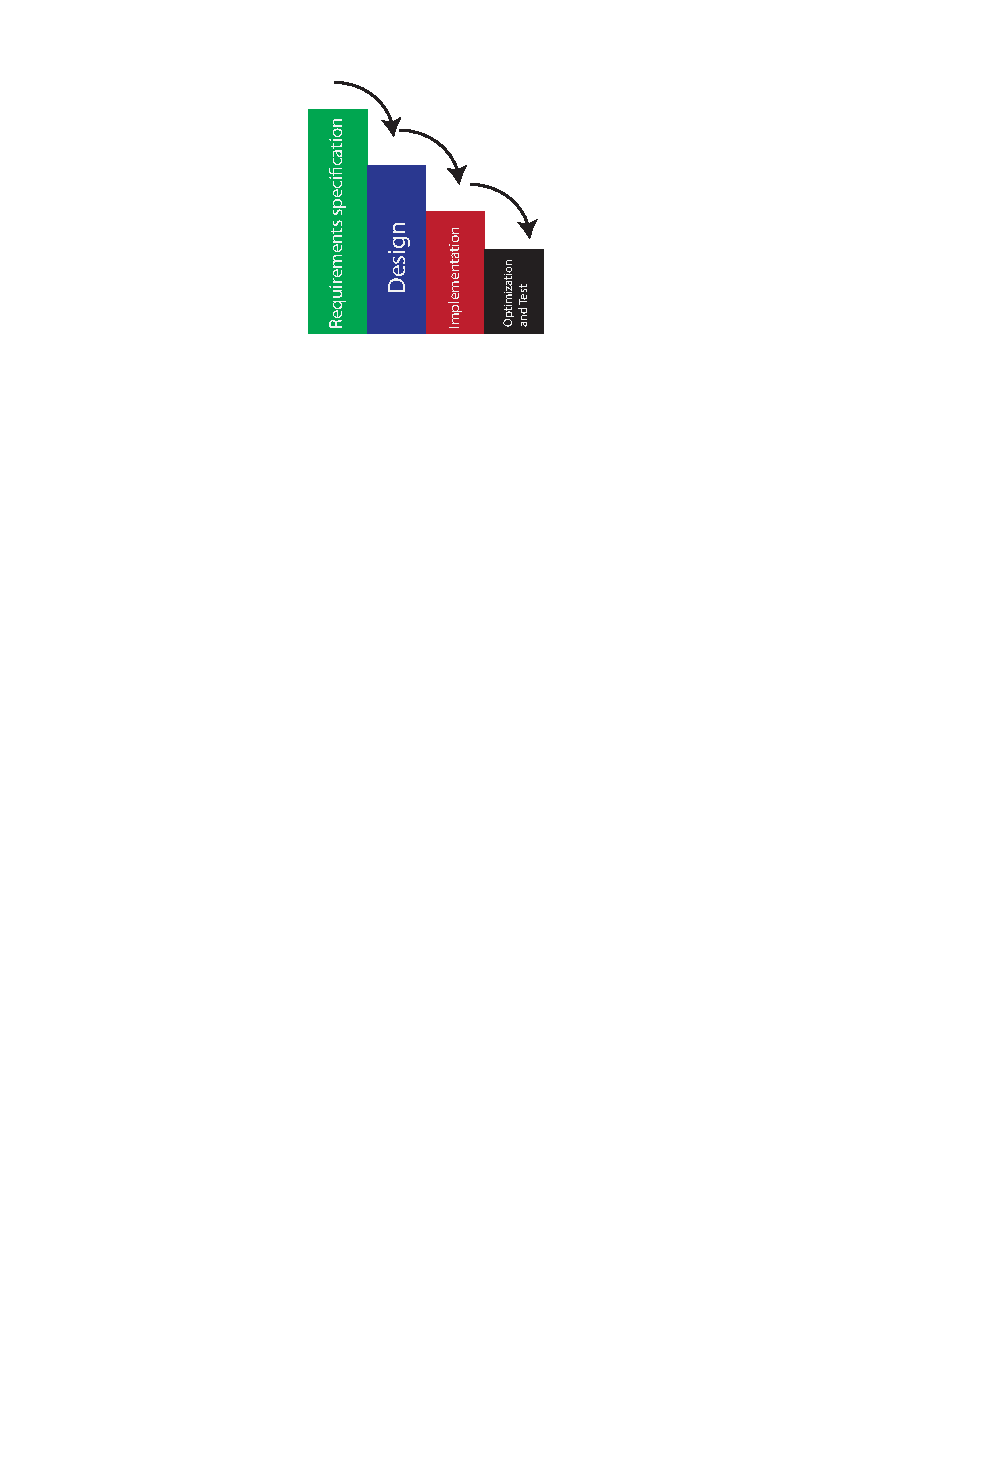
\includegraphics[scale=0.6]{Figures/Waterfall}
\caption{An overview of the waterfall phases.}
\label{fig:Waterfall}
\end{figure}
\newpage

\subsection*{Time Boxing} %Jonathan
We were convinced that using "Time Boxing" would be the way to go. Timeboxing divides The schedule into a number of separate time periods(timeboxes), with each part having its own deliverables, deadline and budget. We used this method to break bigger tasks into smaller tasks with more manageable time frames. What's important is that by the end of each timebox we need are left with a product where if all else fails we can roll back and release our game from an earlier state. The following table shows the timeboxes we have created during the project.
%Please add the following required packages to your document preamble:
%\usepackage[table,xcdraw]{xcolor}
%If you use beamer only pass "xcolor=table" option, i.e. \documentclass[xcolor=table]{beamer}
\begin{table}[h]
\begin{tabular}{llll}
  \rowcolor[HTML]{BBDAFF}
  \textbf{week 8-10}	& \textbf{week 11-13}	& \textbf{week 14-15}	& \textbf{week 16-17}	\\
  Code exercise			& Collision detection	& Level generation		& Graphics				\\
  Class design			& Enemies				& Player				& Level generation		\\
  Game Design			& Input					& 						& Sprites				\\
  \rowcolor[HTML]{BBDAFF} 
  \textbf{week 18}		& \textbf{week 19}		& \textbf{week 20}		& \textbf{week 22}		\\
  Endgame				& Attack				& Animation				& Optimization			\\
  Level generation		& Level generation		& Optimization			& 						\\
  						& Optimization			& Sound					& 						\\
  						& 						& Sprites 				& 						\\
  \rowcolor[HTML]{BBDAFF}
  \textbf{week 23}		& \textbf{week 24}		& \textbf{week 25}		& 						\\
  Attacks				& AI					& Bug Fixes				& 						\\
  Coins					& High score			& Code Polish			& 						\\
  Optimization			& Optimization			& Optimization			& 						\\
\end{tabular}
\caption{The timeplan in timebox format.}
\end{table}

\section{Development Issues} %Cebrail / Jonathan / Carsten
We received the Arduino three weeks after the course started, which was a major setback in implementation. All we could do in this time was design the program structure and time-plans. This skewed our planned agile development. Instead of dynamically designing and implementing additional features, we had to make the most of our time and design for three weeks straight. Usually in agile processes, you make sure to have a working product at the end of each timebox. This was not compatible with our designed framework, since we had taken a lot more features into consideration than possible in a single timebox. It was one very large timebox, more akin to the waterfall process. We could have incrementally implemented the framework after receiving the Arduino, but in the end it would have been slower and more tedious. We had the designs so all we had to do was implement them. In the end we made up for the loss in implementation time by cutting corners in the process and designing a lot ahead.
\newline
Later on, one of the Arduinos burned out. It is not clear what went wrong and it rarely worked. At this time we only had another Leonardo and the Duemilanove. This slowed us down quite a bit as only half of us could program each week. A few weeks later we hit the maximum code size on the Duemilanove, and were left with only a single working Arduino. Development became too slow, until we traded the Duemilanove for another Leonardo.
\newline
General problems with the Arduinos were common. We have also had some issues when uploading code to the Arduino. The screen would be completely black even though the IDE stated the upload was complete. The usual fix was uploading a simple example file from the Arduino library, usually {\tt HelloWorld.ino}. In other cases changing the USB port would solve it. It was probably a sign of incorrect driver installation. Resetting the Arduino during uploading would also sometimes solve it. Other problems were related to the SD card in the Gameduino 2, where we could not upload programs while the SD card was inserted. The SD would get corrupted and a reformatting would be required. Usually this would work, but often only when done through a Mac for unknown reasons.


%Describe the overall structure of the system, the different components of the system and interfaces between these.
\chapter{Overall design}
In this section...\\

\section{Objects} %Carsten
Everything in the game-space is a \emph{prop}. These are the objects which the physics engine works with. Each of them contains a \emph{hitbox}, a rectangular square used to calculate collisions. In addition they also contain graphical information needed to be drawn, since all props should be.\\
Next we have \emph{units}, which would be all enemies and the player. All units are props, and are part of the physics engine. The difference is that a unit has an AI to update too. As a side note, we did not name them actors in suit of the theatrical names, scenes and props, since it would be confusing that all actors are props.\\
The only reason to distinct units and props are because of \emph{coins}. These grant the player a score bonus when collected. The reason for coins to extend props is to reuse collision detection code from props, and makes them affected by the physics engine as a bonus.\\
Two kinds of unit extensions exist: the \emph{minotaur} and the \emph{hero}. The former is the only implemented enemy type in the game and the latter is the unit controlled by the player. These contain graphical and gameplay data as well as their AI code. In case of the hero, his 'AI' is reading player input.

\subsection{Minotaur AI} %Carsten
The AI needs to receive world information and deliver actions. This prompts a cyclic model-controller relationship, which aims to place as much freedom in the hands of the AI as possible. The biggest limiting factor is how complex the world is, most of all the physics engine. The AI cannot and should not predict how its actions would affect the world - this is the job of the physics engine. This limits us in how advanced the AI can be, especially when planning forward, since we cannot guarantee an action leads to the desired outcome. For example, if a unit would jump across a gap or on top of a platform, he would need to steer himself for several frames to land safely and surely. Moreover, planning further than the current frame would require the unit to have a concept of his jumping abilities, size and world geometry.\\
This complexity leads us to create much simpler AI, one which does not plan ahead. A possible solution which was considered, would be preprocessing the map and generate paths through the map. Though this would not be expensive in memory and code-size, and would make different enemy types problematic. Either we would be forced to use similarly moving enemies or generate additional pathing maps for each enemy type. This would be a lot of work for a bit smarter AI, and it was not a very enticing feature with such limited hardware.\\
The AI we settled with would simply move towards a given goal, jumping if necessary, or wander aimlessly like enemies usually do in platforming games.\\
Communication between the unit and the scene is done by an object called \emph{Logic}. This should contain all necessary methods and information needed by all unit types. A few examples would be the hero's position, whether or not a given prop is in the air or whether a given space is 'walkable'. It would also need to execute actions given by the units, which is the physics engine. So it handles collision detection, gravity and calls relevant methods in case a prop collides with a wall or is attacked.\\
As mentioned there is a cycle of dependencies: Logic requires scenes for map information, which includes units, which need logic to communicate. We attempted to avoid cycles which could be a problem during implementation, but it seemed unavoidable when an informed AI is in play.

\subsection{Hero Input}
Both Arduino and the Gameduino 2 shield gives us opportunities to control the game. Arduino can communicate with a pc and get data when a key is pressed on the keyboard. The Gameduino 2 is equipped with a touch screen and a accelerometer. We could have used one of these to get input, but none of them gives a natural way to play a 'platformer` on a Gameduino 2. The pc solution feels not natural as the keyboard and the Gameduino 2 screen usually are not in front of each other. The touch screen is not as responsive as we wanted, and it would also be annoying as the fingers will get in the way. The accelerometer is just wrong in all way, it is hard to control, as you always has to 'feel' how to hold the device. The problem with fingers getting in the way appears also here. The best option was using a external controller - a Wii nunhcuk.

\begin{figure}[h] 
  \centering 
  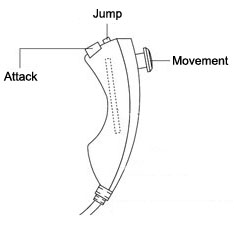
\includegraphics[scale=0.6]{Figures/nunchuk}
  \caption{Button assignments}
  \label{fig:Nunchuk} 
\end{figure}

We assigned the thumbstick to move horizontally and duck. The two buttons at the top are used to jump and attack. These buttons assignments was the combination that felt most comfortable.

\section{Levels} %Carsten
The levels in the game are called \emph{scenes}. They contain the world geometry and all the props. The world is made out of square blocks called \emph{tiles}. There are multiple types of tiles, used to diversify the world and mark special locations. The former kind is solid blocks and partially solid platforms, while the latter is the entrance and exit. The scene is composed of a \emph{grid} of tiles which contains exactly one entrance and exit. Each level is a climb to the top, with the entrance at the bottom and exit at the top. Minotaurs and coins are randomly placed around the map, though not too close to the entrance.\\
Initially, ladders were also supposed to be in the game, but their function would have overlapped with platforms. Ladders would be difficult to implement and would require specific animations, both for the player and the enemies. They were cut from the game in favor of the easier to implement platforms.

\subsection{Generated Maps}

\section{Graphics}
Gameduino...

\subsection{Assets}
Assets...

\subsection{Sound} %Cebrail/Jonathan

We implemented sound effects on essential events. We Agreed that it was what the game needed to give a better feel.\\
We decided that the sounds we wanted was from the hero, and when he interacts with something. We added a sounds for jumping, attacking, when exiting a map and when collecting a coin.\\
To include bacground music we would have needed about 2kb more space in the flash memory since it takes alot of code to make this work. A solution would have been to use a shorter music file in the GD2 file and looping it, but we agreed that it would be annoying and steered clear of it.



\chapter{Hardware} %Cebrail

During the project we have worked with two Arduino types. Duemilanove and Leonardo clone.
The clone was more powerful and therefore was our main used board. The clone is called
OLIMEXINO-32U4.
\subsection{Specications}

\subsubsection{Arduino}
The specs of the Arduino boards vary very much of each other. The OLIMEXINO is definitely
better.

\begin{table}[h]
\resizebox{16cm}{!} {
    \begin{tabular}{l|l|l|l|l|l|l}
    Board name     & Microcontroller & Operating Voltage & Flash Memory & Clock Speed & Input Power & SRAM   \\ \hline
    OLIMEXINO-32U4 & ATMEGA32U4      & 3.3V / 5V         & 32KB         & 16 MHz      & 7-12VDC     & 2.5 KB \\
    Duemilanove    & ATmega168       & 5V                & 16 KB        & 16 MHz      & 7-12V       & 1 KB   \\
    \end{tabular}
}
    \caption{Specifications of the boards}
\end{table}

\subsubsection{Gameduino2}
The specificatins of the Gameduino2\footnote{http://excamera.com/sphinx/gameduino2/} shield.

\begin{itemize}
  \footnotesize
  \item Video output is 480x272 pixels in 24-bit color.
  \item OpenGL-style command set.
  \item Up to 2000 sprites, any size.
  \item 256 Kbytes of video RAM.
  \item Smooth sprite rotate and zoom with bilinear filtering.
  \item Smooth circle and line drawing in hardware - 16x antialiased.
  \item JPEG loading in hardware.
  \item Built-in rendering of gradients, text, dials and buttons.
\end{itemize}


\subsection{input}
The Wii nunchuk is one of the ways to control the game, aside from the
touchscreen.
The nunchuk has to be connected to the Arduino by hardware. Even though they
use same slots in the board, it is possible to use both the Gameduino 2 and Wii
nunchuk at the same time because they use different hardware interfaces. The
Gameduino uses an ISP interface, while the Wii nunchuk uses an I2C interface.
The Gameduino requires 5 volt to work, which forces us may shorten the lifetime
of the nunchuk - as it normally operates at 3.3 volt, but it should not be a
big concern.


\begin{figure}[h]
\centering
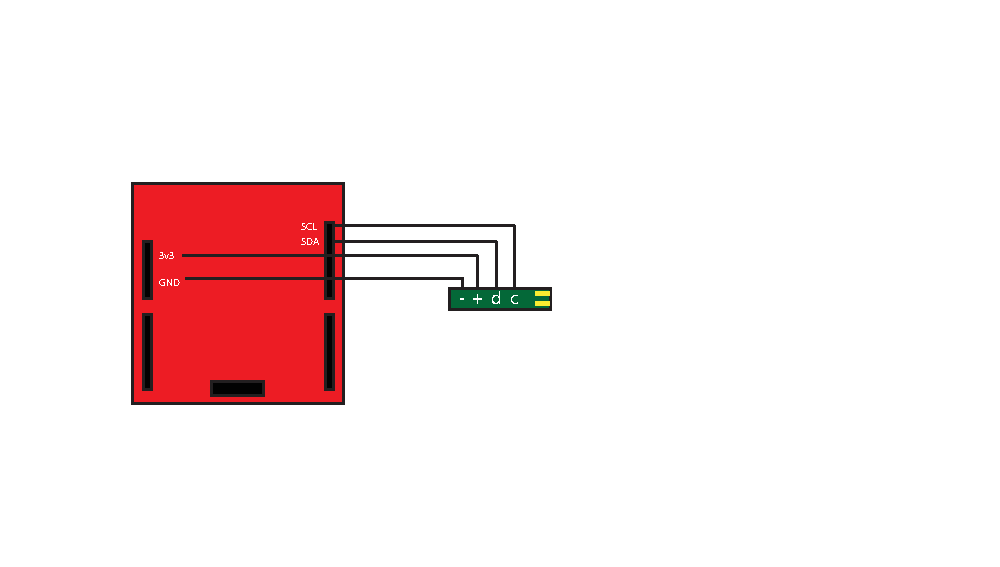
\includegraphics{Figures/NunchuckConnection}
\caption{Hardware connection of an nunchuk}
\label{fig:nunchuk_connect}
\end{figure}


\subsection{I2C}
The I2C is the interface, which is used by the Wii nunchuk adapter. This bus
interface allows easy communication between components and only requires two
bus lines. These lines are both bidirectional. These bus lines are called SCL
(Serial Clock Line) and SDA (Serial Data Line).


\begin{figure}[h]
\centering

\includegraphics[scale=0.4]{Figures/I2C}
\caption{Hardware connection of an nunchuk}
\label{fig:i2c}
\end{figure}


\begin{enumerate}
\item Data trans fer is initiated with a START bit (S) signaled by SDA being
pulled low while SCL stays high.
\item SDA sets the 1st data bit level while keeping SCL low (during blue bar
time.) and the data is sampled (received) when SCL rises (green).
\item When the transfer is complete, a STOP bit (P) is sent by releasing the
data line to allow it to be pulled high while SCL is kept high continuously.
\item In order to avoid false marker detection, the level on SDA is changed on
the SCL falling edge and is sampled and captured on the rising edge of SCL.
\end{enumerate}










\include{Implementation}

%\section{Testing and performance analysis}
\chapter{Testing and performance analysis}

Present test methodology as well as results in this section.
In addition, if performance analysis of the system is interesting, present it here as well.

A few screenshots of the program can be included here as well.




\chapter{Discussion}
 
One of our biggest problems here towards the end has been the amount of flash memory. This set a limit for what we could add and how we could add it. Some places in our code we have had to implement some things rather crudely to save flash memory, an example is that we have not used any getters/setters all is done with public variables. We have also had problems the amount we could store on our GD2 file this limited us to a few selected sprites and audio files.

Furthermore we have had some issues with spawning coins.\\

Additional features could be implemented but that would require a board with more memory. If this was the case we could implement the features we wanted originally, story, more monsters, items, levels and so on.\\
We have been very limited by the boards capacities. But this has taught us to work with code another way than we usually do. Today when making a platformer for computer we will never reach a point where we have too much code, but how compact is the code, how optimized is it? instead of optimizing you would just build additional features once the last feature worked. Since none of us had experience with c++ we have struggled a bit with the documentation on the arduino site and the "guide book" from the GD2 library. We have had some cases where the documentation has been plain wrong, and mostly confusing and badly written with bad examples.


\section{Meeting Requirements}

\subsection*{Cut content}
Items, merchant and levels
increasing difficulty?
Multiple enemies?
\subsection*{Additional content}
More or less advanced physics engine.
Coin physics.


%\section{Conclusion}
\chapter{Conclusion}

Summarize the main results. This section should make sense even if the reader has only read the introduction.




\newpage

\textbf{References}

\subsection{Links}


I2C Interface: \url{http://en.wikipedia.org/wiki/I%C2B2C}

\newpage
%\section{Appendices}
\chapter{Appendices}


\subsection{Optimization}
\begin{figure}[h]
  \centering
  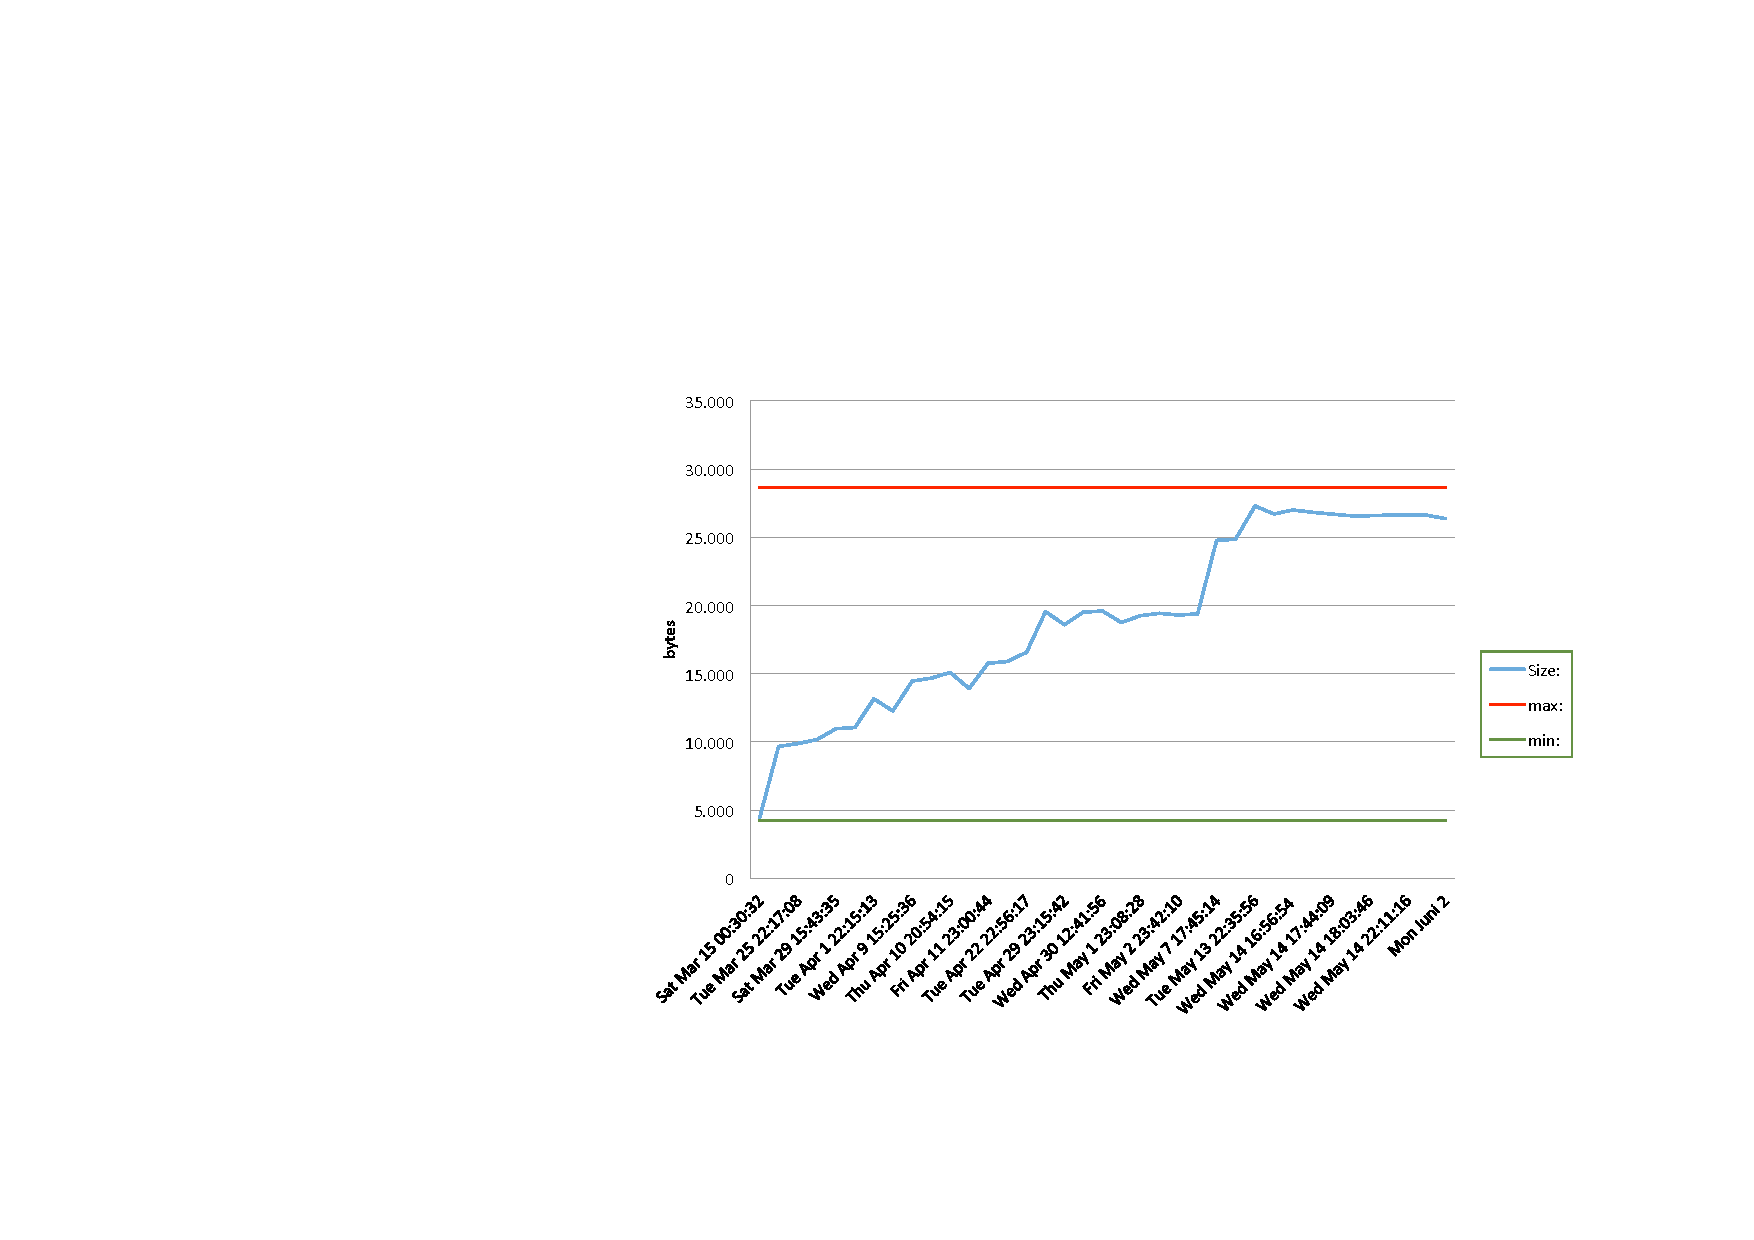
\includegraphics[scale=0.8]{Figures/CodeSizeChart}
  \caption{A history of the code size}
  \label{fig:code_size}
\end{figure}
\newpage
\subsection{Requirements}
\begin{figure}[h]
  \centering
  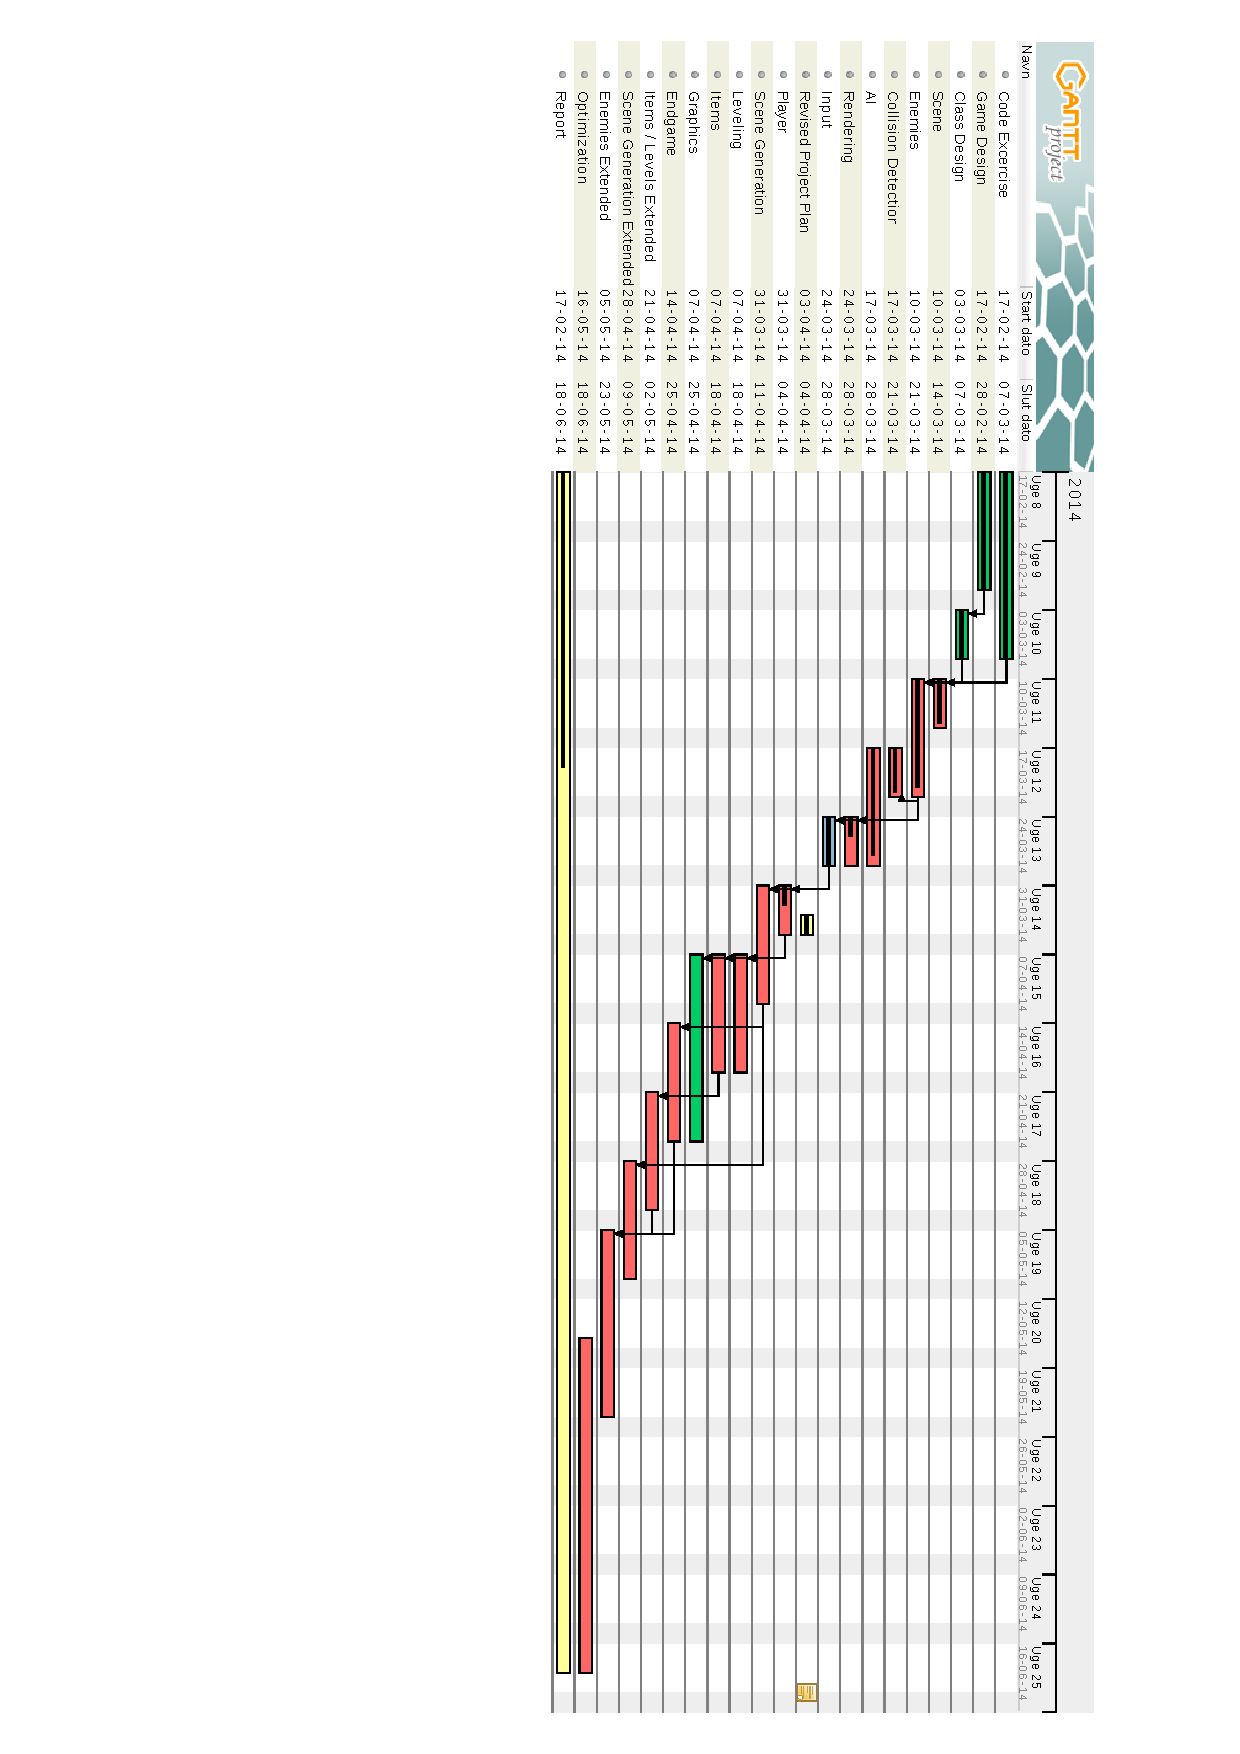
\includegraphics[scale=0.55]{Figures/Tidsplan2}
  \caption{The waterfall timeplan of our project}
  \label{fig:Waterfall_chart}
\end{figure}
\end{document}
